The above two line equations can be expressed as the matrix equation
    \begin{align}
    \myvec{4 & 7\\2 & -3 }{\vec{x}} = \myvec{3\\-1 }
    \end{align}
    Constructing the augmented matrix

    \begin{align}
    \myvec{4 & 7 & 3 \\ 
        2 & -3 & -1 }
    \end{align}

    Transforming the matrix into row-echelon form
    \begin{align}
    \myvec{
    4 & 7 & 3 \\
    2 & -3 & -1
    }
      \xleftrightarrow[]{R2 \leftarrow 2R2 - R1 } \nonumber \\
    \myvec{
    4 & 7 & 3 \\
    0 & -13 & -5
    }
    \xleftrightarrow[]{R2 \leftarrow -R2/13,R1 \leftarrow R1/4} \nonumber \\
    \myvec{
    1 & 7/4 & 3/4 \\
    0 & 1 & 5/13
    }
    \xleftrightarrow[]{R1 \leftarrow R1-7/4R1/4} \nonumber \\
    \myvec{
    1 & 0 & 2/26 \\
    0 & 1 & 5/13
    }
    \end{align}
    The solution for x can be written as 
    \begin{align}
    \label{expk}
    \vec{x} = \myvec{2/26 \\ 5/13}
    \end{align}
    Thus, The point of intersection is at point (2/26 , 5/13) i.e. (0.07, 0.38)\\
    Let the equation of the line be
    \begin{align}
    \label{equ}
    \vec{n}^T\vec{x} = c \implies \vec{x}^T\vec{n} = c
    \end{align}
    Let the intercepts be a,b on the x and y axis respectively. Then,
    \begin{align} 
    \myvec{a & 0}\vec{n} = c
    \end{align}
   
    \begin{align} 
    \myvec{0 & b}\vec{n} = c
    \end{align}
    resulting in the matrix equation
    \begin{align}
    \myvec{a & 0 \\ 0 & b}\vec{n} = c \myvec{1 \\ 1}
    \end{align}
    As the intercepts are equal,Let a=b
    \begin{align}
    \myvec{a & 0 \\ 0 & a}\vec{n} = c \myvec{1 \\ 1}
    \end{align}
    \begin{align}
    \vec{n} = \frac{c}{a}\myvec{1\\1} = \myvec{1\\1}
    \end{align}
    As the line passes through point of intersection,We can use the equation \eqref{expk} in equation \eqref{equ} to find the value of c\\
    \begin{align}
    c=
    \myvec{1 & 1}
    \myvec{\frac{2}{26} \\  
    	\frac{2}{26} }
    \end{align}
    \begin{align}
    \implies c=\frac{2}{26}+\frac{2}{26}
    \implies c=\frac{6}{13}
    \end{align}
    So, the equation of line can be written as
    \begin{align}
    \implies
    \myvec{1 & 1}
    	{\vec{x}} = \frac{6}{13}
    \end{align}
    \begin{figure}[!ht]
    \centering
    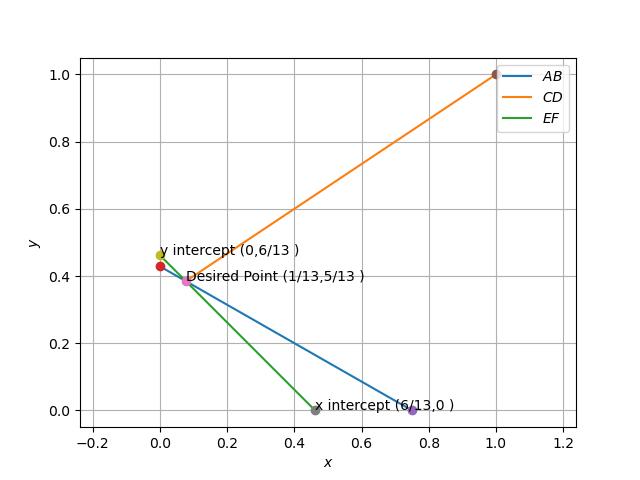
\includegraphics[width=\columnwidth]{./solutions/line_plane/50/Assignment_1}
     \caption{The intercepts of the required line are equal}
\label{fig:solutions/line_plane/50/}
    \end{figure}
